\section{Temel kavramlar}\label{sec:kavram}

Bu bölüm, proje boyunca duyacağınız her terimi sıfırdan anlatır. Zorlanırsanız Ek~\ref{ek:sozluk}'teki sözlüğe bakın.

\subsection{5G NR radyo kaynak ızgarası}\label{sec:grid}

5G NR'de radyo kaynağı bir \textbf{zaman--frekans ızgarasıdır}:
\begin{itemize}
\item \textbf{Zaman ekseni:} bir \textbf{slot} 14 \textbf{OFDM sembolünden} oluşur. Slot süresi alt taşıyıcı aralığına (SCS) bağlıdır:
  15\,kHz'de 1\,ms, 30\,kHz'de 0,5\,ms.
\item \textbf{Frekans ekseni:} 12 alt taşıyıcı bir \textbf{PRB}'yi (Physical Resource Block) oluşturur. 20\,MHz'lik, 15\,kHz'lik bir hücrede yaklaşık 106 PRB vardır.
\item En küçük birim \textbf{kaynak elemanı (RE)}: 1 sembol $\times$ 1 alt taşıyıcı.
\end{itemize}

Izgaranın her bölgesinin bir görevi vardır:

\begingroup\sffamily\small
\begin{xltabular}{\textwidth}{@{}p{2.2cm}X@{}}
\toprule
\textbf{Kanal/sinyal} & \textbf{Görevi} \\
\midrule
PDSCH & Kullanıcı verisi (indirme, \emph{downlink}). Throughput'u belirleyen kaynak. \\
PDCCH & Kontrol: hangi kullanıcı hangi PRB'yi alıyor? Slotun ilk sembollerinde. \\
SSB & Senkronizasyon: telefonlar hücreyi bulsun diye periyodik yayın. \\
PRS & \textbf{Konumlandırma referans sinyali} (Rel-16). Bilinen bir dizi içerir, bu yüzden \emph{radar gibi} kullanılabilir. \\
SRS & Telefonun gönderdiği (yukarı bağlantı) referans sinyali. Kanal ölçümü için. \\
\bottomrule
\end{xltabular}
\endgroup

\begin{figure}[H]
\centering
\includegraphics[width=0.88\textwidth]{sekiller/fig_grid.pdf}
\caption{Şematik kaynak ızgarası (8 slot). Turuncu bloklar slot 1 ve 5'teki sensing/PRS sinyali: kapladığı PRB'ler o slotta kullanıcı verisi için kullanılamaz.
Bu şema OCUDU'da PRS periyodu $T=4$ slot ve ofset 1 olan gerçek bir yapılandırmayı temsil eder.}
\label{fig:grid}
\end{figure}

\textbf{Sensing bu ızgarada nasıl görünür?} Sensing için gönderilen sinyal (örneğin PRS), ızgaranın bir bölgesini kaplar. Orası artık kullanıcı verisi taşıyamaz.
Ne kadar bölge kaplandığı, \textbf{sensing kaynak payı} $\alpha$'dır. Bu projenin merkezindeki sayı budur.

\subsubsection{Zihninde canlandır: ızgara bir tablodur}\label{sec:somut}

Izgarayı \textbf{bir Excel tablosu} gibi düşün: \emph{sütunlar zaman} (semboller), \emph{satırlar frekans} (alt taşıyıcılar). Scheduler bu tabloyu her slotta
\textbf{dikdörtgenlere böler}; her dikdörtgen bir kullanıcının verisidir (ya da bir sinyaldir: SSB, PRS...). Aşağıda önce tablonun ölçeğini, sonra \emph{gerçek bir gNB'nin} bu tabloyu nasıl doldurduğunu göreceksin.

\begin{figure}[H]
\centering
\begin{tikzpicture}[node distance=5mm and 11mm,font=\sffamily\small]
  \node[ndn,text width=1.9cm] (a) {\textbf{1 saniye}};
  \node[nd,text width=2.3cm,right=of a] (b) {\textbf{çerçeve}\\[-1pt]{\scriptsize 10\,ms}};
  \node[nd,text width=2.3cm,right=of b] (c) {\textbf{slot}\\[-1pt]{\scriptsize 1\,ms}};
  \node[nd,text width=2.6cm,right=of c] (d) {\textbf{OFDM sembolü}\\[-1pt]{\scriptsize $\approx$ 71\,$\mu$s}};
  \draw[ar] (a) -- node[lab,above] {$\times100$} (b);
  \draw[ar] (b) -- node[lab,above] {$\times10$} (c);
  \draw[ar] (c) -- node[lab,above] {$\times14$} (d);
  \node[ndg,text width=2.4cm,below=9mm of a] (e) {\textbf{alt taşıyıcı}\\[-1pt]{\scriptsize 15\,kHz}};
  \node[ndg,text width=2.3cm,right=of e] (f) {\textbf{PRB}\\[-1pt]{\scriptsize 180\,kHz}};
  \node[ndg,text width=2.3cm,right=of f] (g) {\textbf{tüm hücre}\\[-1pt]{\scriptsize $\approx$ 19\,MHz}};
  \draw[ar] (e) -- node[lab,above] {$\times12$} (f);
  \draw[ar] (f) -- node[lab,above] {$\times106$} (g);
  \node[lab,anchor=east] at ([xshift=-4mm]e.west) {\textbf{frekans}};
  \node[lab,anchor=east] at ([xshift=-4mm,yshift=9mm]e.west) {\textbf{zaman}};
\end{tikzpicture}
\caption{Zaman ve frekans eksenlerinde ``kaç tane ne'' (15\,kHz alt taşıyıcı aralığı, 20\,MHz'lik hücre). Slotun içinde 14 sütun (sembol) ve $106\times12=1272$ satır (alt taşıyıcı) vardır.}
\end{figure}

\paragraph{Bir slotun kaç kaynak elemanı var?}
\begin{equation*}
\underbrace{106}_{\text{PRB}}\times\underbrace{12}_{\text{alt taşıyıcı/PRB}}\times\underbrace{14}_{\text{sembol}}=\mathbf{17\,808}\ \text{kaynak elemanı (RE) / slot}
\end{equation*}
Saniyede 1000 slot olduğundan bu, saniyede $\approx 17{,}8$ milyon RE eder. Bir RE 64QAM ile en çok 6 bit taşıyabilir; bu yüzden teorik üst sınır slot başına $17\,808\times 6=106\,848$ bit,
yani yaklaşık 107\,Mbps'tir. Gerçek sistem bunun altında kalır, çünkü kontrol sinyalleri, referans sinyalleri ve hata düzeltme kodu yer kaplar.

\paragraph{Gerçek bir gNB bu tabloya ne yazıyor?}
OCUDU'yu çalıştırıp scheduler log'unu açtık (PRS her 4 slotta bir; \texttt{ogretici/betikler/ocudu\_slot\_log.sh}). Log'dan \emph{gerçek} iki satır:

\begin{lstlisting}
[  876.7] PDSCH: rnti=0x44 ... prb=[0, 96) symb=[1, 14) mod=64QAM ... tbs=7941
[  880.1] PUSCH: rnti=0x44 ... prb=[0, 106) symb=[0, 14) mod=64QAM ... tbs=9737
\end{lstlisting}

Bu tek satırı ``ızgara tablosu'' diliyle oku:
\begin{center}
\sffamily\small
\begin{tabularx}{\textwidth}{@{}p{3.3cm}p{4.6cm}X@{}}
\toprule
\textbf{Log'da} & \textbf{Anlamı} & \textbf{Tabloda nereye karşılık gelir?} \\
\midrule
\texttt{[ 876.7]} & Çerçeve 876, slot 7 & 876. çerçevenin (10\,ms) 8. slotu (15\,kHz'de bir çerçevede 10 slot var). \\
\texttt{prb=[0, 96)} & PRB 0'dan 95'e: \textbf{96 PRB} & Tablonun \emph{frekans} yönündeki kalınlığı: $96\times12=1152$ alt taşıyıcı. \\
\texttt{symb=[1, 14)} & Sembol 1'den 13'e: \textbf{13 sembol} & Tablonun \emph{zaman} yönündeki uzunluğu. Sembol 0 kontrol kanalına (PDCCH) kalır. \\
\texttt{mod=64QAM} & 64QAM modülasyon & Her RE 6 bit taşır (en çok). \\
\texttt{tbs=7941} & Taşıma bloğu: \textbf{7941 bayt} & Bu dikdörtgenin taşıdığı veri: $7941\times8=63\,528$ bit. \\
\bottomrule
\end{tabularx}
\end{center}

Yani bu kullanıcıya verilen dikdörtgen $96\times12\times13=\mathbf{14\,976}$ RE'dir ve $63\,528$ bit taşır:
RE başına $63\,528/14\,976\approx 4{,}24$ bit (6 bitten az, çünkü DMRS referans sinyali ve kodlama yeri tutar). Slot başına $\approx 63{,}5$\,kbit ve saniyede 1000 slot $\Rightarrow$ en çok $\approx 63{,}5$\,Mbps.

\begin{bulgu}[Throughput'u elle hesapladık, ölçümle tuttu]
Log'daki 6365 PDSCH'nin ortalama taşıma bloğu 7251 bayt, yani \textbf{58,0\,kbit/slot} (en çok kullanılan kalıp: 96 PRB, bazen 40 PRB).
\begin{itemize}[leftmargin=1.4em]
\item \textbf{PRS yokken:} saniyede 1000 PDSCH'li slot $\Rightarrow 1000\times58{,}0=58{,}0$\,Mbps. Ölçülen: \textbf{59,0\,Mbps}.
\item \textbf{PRS her 4 slotta bir iken:} saniyede 750 PDSCH'li slot $\Rightarrow 750\times58{,}0=43{,}5$\,Mbps. Ölçülen: \textbf{43,8\,Mbps}.
\end{itemize}
\textbf{Kural:} DL throughput $\approx$ (PDSCH'li slot sayısı / s) $\times$ (taşıma bloğu bit/slot). Sensing bu çarpımın birinci çarpanını (PDSCH'li slot sayısı) ya da ikincisini (PRB sayısı) küçültür. Projenin özü bu iki cümledir.
\end{bulgu}

\begin{figure}[H]
\centering
\includegraphics[width=0.98\textwidth]{sekiller/fig_slot_serit.pdf}
\caption{\textbf{Gerçek OCUDU log'undan 40 ardışık slot} (SFN 890.0'dan 893.9'a; veri: \texttt{ogretici/veri/ocudu\_slot\_serit.csv}). Her çubuk bir slotu, yüksekliği PDSCH'ye verilen PRB sayısını gösterir.
\textbf{Turuncu slotlarda PDSCH hiç yok:} bunlar 890.1, 890.5, 890.9, \ldots, yani \emph{tam her 4. slot}. PRS periyodunu 4 slot, ofsetini 1 yapmıştık.
Sarı slotlar (\texttt{.0}) yalnızca 40 PRB alıyor; muhtemelen aynı slottaki SSB yer tuttuğu için (bunu kodla doğrulamadık).}
\label{fig:slot-serit}
\end{figure}

Bu şekil bölümün en önemli görseli: \textbf{PRS'in ``kaynağı götürmesi'' soyut bir cümle değil, log'da sayılabilir bir şeydir}: her 4. slotta tablonun tamamı PRS'e gider, o slotta kullanıcıya hiçbir şey kalmaz.
Ayrıca \texttt{symb=[1, 14)} her PDSCH'de aynı: veri hep slotun \emph{tamamına} yayılıyor. Bu, Bölüm~\ref{sec:prs}'deki ``4 sembollük PRS de 12 sembollük PRS kadar kayıp veriyor'' bulgusuyla uyumlu bir açıklama olabilir
(PRS'in kapladığı PRB'lere slotun bütününde veri verilemiyor), ama bunu henüz kodla doğrulamadık.

\begin{figure}[H]
\centering
\includegraphics[width=0.96\textwidth]{sekiller/fig_izgara_kareler.pdf}
\caption{\textbf{Aynı veri, bu kez ızgara olarak:} 8 ardışık slotun her biri 14 sembol $\times$ 106 PRB'lik bir tablo. Mavi dikdörtgen log'daki PDSCH tahsisidir (\texttt{prb}, \texttt{symb} değerleri log'dan). Turuncu dikdörtgen yapılandırmadaki PRS'tir (periyot 4, ofset 1, 12 sembol, 104 PRB). Soluk yeşil şerit: PDSCH'nin başlamadığı sembol 0 (kontrol alanı). Animasyonlu hâli: \texttt{ogretici/sekiller/ocudu\_izgara\_filmi.gif}.}
\end{figure}

\begin{pilot}[Kendin dene (20 dakika)]
\begin{enumerate}[leftmargin=1.5em]
\item \textbf{Elle hesapla:} Alt taşıyıcı aralığı 15 yerine \textbf{30\,kHz}, bant 20 yerine \textbf{40\,MHz} olsun. Bu durumda PRB sayısı yine 106'dır (3GPP TS 38.101-1'deki tabloya göre; sen de tabloya bakıp doğrula, biz doğrulamadık).
  (a) Bir slot kaç ms sürer, saniyede kaç slot vardır? (b) Bir slotun RE sayısı değişir mi? (c) Saniyedeki RE sayısı kaç kat artar? (d) Bir PRB artık kaç kHz'dir?
  \emph{Beklenen cevap:} (a) 0,5\,ms, 2000 slot/s. (b) Hayır, 17\,808. (c) 2 kat ($\approx 35{,}6$ milyon RE/s). (d) $12\times30=360$\,kHz.
\item \textbf{Gerçeği gör:} Ubuntu'da \texttt{bash ogretici/betikler/ocudu\_slot\_log.sh} çalıştır. Sonra \texttt{grep -a "PDSCH: rnti" /tmp/gnb\_slotlog.log | head} ile ilk PDSCH satırlarını bul ve yukarıdaki tabloyla okumayı dene: \texttt{prb}, \texttt{symb}, \texttt{tbs} ne diyor?
\item \textbf{PRS slotlarını bul:} \texttt{grep -a "Slot decisions" /tmp/gnb\_slotlog.log | head -50} satırlarında \texttt{0 PDSCHs} geçen slotların numaralarına bak. Aralarındaki fark kaç? (Cevap: 4.)
\item \textbf{Değiştir:} \texttt{ogretici/veri/ocudu\_p4\_config.yml} dosyasında \texttt{periodicity\_slots: 8} yap, tekrar çalıştır. \texttt{0 PDSCHs} slotları şimdi kaç slotta bir? Throughput ne olur?
\end{enumerate}
\end{pilot}

\subsection{gNB'nin iç yapısı: CU, DU, RU}\label{sec:gnb}

Bir gNB tek parça değildir. Açık RAN mimarisinde (O-RAN) işlevler katmanlara bölünür:

\begin{figure}[H]
\centering
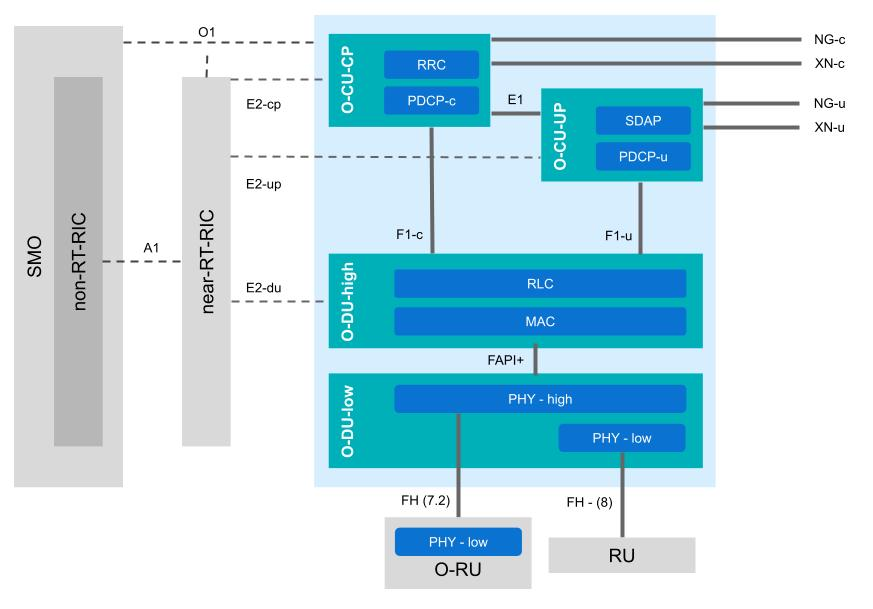
\includegraphics[width=0.78\textwidth]{sekiller/oran_gnb_arch.jpg}
\caption{O-RAN gNB mimarisi. Kaynak: OCUDU deposu, \texttt{lib/oran\_gnb\_arch.jpg} (SPDX: BSD-3-Clause-Open-MPI, Software Radio Systems Limited).
Biz özellikle \textbf{O-DU-high} içindeki \textbf{MAC} (scheduler orada) ve \textbf{O-DU-low}'daki \textbf{PHY} ile ilgileniyoruz.}
\label{fig:oran}
\end{figure}

\begingroup\sffamily\small
\begin{xltabular}{\textwidth}{@{}p{2.3cm}X@{}}
\toprule
\textbf{Parça} & \textbf{Ne yapar?} \\
\midrule
CU-CP / CU-UP & Merkezi birim: kontrol düzlemi (RRC, bağlantı yönetimi) ve kullanıcı düzlemi (veri yönlendirme, SDAP/PDCP). Çekirdek ağla konuşur. \\
DU-high & RLC ve \textbf{MAC}. MAC'in içindeki \textbf{scheduler}, her slotta kaynakları kullanıcılara dağıtır. \\
DU-low & PHY (fiziksel katman): modülasyon, kodlama, FFT. PRS sinyalini üreten kod burada. \\
RU & Radyo: antenler ve RF. Bizde gerçek RU yok; yazılımla taklit ediliyor (\texttt{ru\_dummy}, ZMQ). \\
\bottomrule
\end{xltabular}
\endgroup

\subsection{Scheduler: slotta kim ne alır?}\label{sec:sched}

\textbf{Scheduler}, \emph{her slotta} (örneğin her 1\,ms) bir karar verir: hangi kullanıcı hangi PRB'leri, hangi modülasyonla alacak?
Bu kararın sonucu bir ``tahsis listesi''dir. Çok kullanıcılı bir ağda throughput'u ve gecikmeyi esas olarak scheduler belirler.

Yaygın politikalar:
\begin{itemize}
\item \textbf{Round-Robin (RR):} herkese sırayla.
\item \textbf{Proportional Fair (PF):} kanalı iyi olana öncelik verir ama kimseyi aç bırakmaz. En yaygın politika.
\item \textbf{QoS-farkında (örn.\ M-LWDF, EXP/PF):} gecikme bütçesi yaklaşan paketlere öncelik. (Capozzi vd.~\cite{capozzi}'nin taraması bu aileyi anlatır.)
\end{itemize}

\textbf{Neden önemli?} Sensing sinyali, scheduler'ın dağıtabileceği kaynak havuzundan düşer. Yani sensing bir \emph{scheduler problemi}dir:
sensing kaynaklarını önceden mi ayırırız, yoksa yük arttıkça mı küçültürüz?

\subsection{OFDM radar: yankıdan menzil ve hız}\label{sec:radar}

OFDM sinyali (5G'nin kullandığı) bir radar olarak da çalışır. Fikir şu:

\begin{enumerate}
\item gNB bilinen bir OFDM sinyali gönderir ($X$).
\item Hedeften yansıyan sinyal ($Y$) gecikmiş ve Doppler kaymış olarak geri gelir.
\item $H = Y/X$ (kanal tahmini) hesaplanır. Alt taşıyıcılar arasındaki \textbf{faz eğimi gecikmeyi (menzili)}, semboller arasındaki \textbf{faz eğimi Doppler'i (hızı)} verir.
\item Bir \textbf{2 boyutlu FFT} bu iki eğimi bir \textbf{range-Doppler haritasına} çevirir. Hedef haritada bir tepe noktası olarak görünür.
\end{enumerate}

\begin{figure}[H]
\centering
\includegraphics[width=0.78\textwidth]{sekiller/fig_rd_map.pdf}
\caption{\textbf{Simülasyon:} iki hedefli (120\,m, +25\,m/s ve 260\,m, $-18$\,m/s) bir OFDM radarın range-Doppler haritası.
Parametreler TR 38.765 Ek~A ile uyumlu: 4,9\,GHz, 30\,kHz SCS, 1024 alt taşıyıcı ($\approx$ 30,7\,MHz), 128 sembol. Halkalar gerçek konumdur; tepeler halkaların içine düşer.
Betik: \texttt{ogretici/betikler/make\_figs.py}.}
\label{fig:rd}
\end{figure}

\textbf{Çözünürlük}, iki hedefi ayırt etme yeteneğidir ve iki şeye bağlıdır:
\begin{equation}
\Delta R=\frac{c}{2W},\qquad \Delta v=\frac{\lambda}{2\,M\,T_{sym}}
\end{equation}
$W$: sensing sinyalinin bant genişliği, $M$: gözlenen OFDM sembol sayısı, $T_{sym}$: sembol süresi, $\lambda$: dalga boyu.
Bu denklemler Lin~\cite{lin}'in IV.\ bölümünde ve Dickerson vd.~\cite{dickerson}'in Tablo~II'sinde de geçer.

\begin{figure}[H]
\centering
\includegraphics[width=0.92\textwidth]{sekiller/fig_resolution.pdf}
\caption{Çözünürlük, sensing'e verdiğimiz kaynakla belirlenir. \textbf{Daha çok bant ($W$) $\rightarrow$ daha ince menzil.
Daha çok sembol ($M$) $\rightarrow$ daha ince hız.} Bu yüzden ``sensing'e kaynak vermek'' sensing kalitesinin doğrudan sebebidir.}
\end{figure}

\begin{pilot}[Kendi gözünle gör]
\texttt{kurulum\textbackslash sionna\_dogrulama.py} dosyasını çalıştırın. Gerçek hedef 120\,m ve 25\,m/s'ydi; betik hedefi 122,1\,m ve 25,9\,m/s olarak buldu.
Hata, çözünürlük hücresinin (4,88\,m, 6,47\,m/s) içinde. \textbf{Soru:} bant genişliğini 4~kat artırsak menzil hatası ne olur? (Cevap: yaklaşık 4~kat azalır, formülden.)
\end{pilot}

\subsection{Sensing sinyali olarak ne kullanılır?}\label{sec:sinyal}

Sensing için yeni bir sinyal icat etmek yerine, 5G'de zaten olan ve alıcının \emph{önceden bildiği} sinyaller kullanılır
(bilinen bir sinyal olmazsa $H=Y/X$ hesaplanamaz):

\begingroup\sffamily\small
\begin{xltabular}{\textwidth}{@{}p{2cm}XX@{}}
\toprule
\textbf{Sinyal} & \textbf{Avantaj} & \textbf{Sorun} \\
\midrule
PRS (DL) & Geniş bant, seyrek yapılandırılabilir, standart (Rel-16). Radar için en çok çalışılan aday \cite{wei,nist,khos}. & Comb yapısı \emph{hayalet hedef (ghost target)} üretebilir \cite{khos}. \\
DMRS (DL, PDSCH içinde) & Veri sinyaliyle birlikte gelir: sensing neredeyse bedava. & Seyrek, yalnızca veri olan yerde var. \\
SRS (UL) & Telefon gönderir; bistatic/pasif sensing mümkün \cite{gurung}. & Telefonun gücü ve zamanlaması sınırlı. \\
Özel sinyal (örn.\ ZC) & Tasarım serbest, iyi korelasyon. & Standartta yok; ek kaynak ister \cite{dickerson}. \\
\bottomrule
\end{xltabular}
\endgroup

\textbf{OCUDU'da PRS zaten var} (Bölüm~\ref{sec:ocudu}): hem MAC'te zamanlayıcısı hem PHY'de üretici kodu mevcut. Bu, projenin en önemli teknik bulgularından biridir.

\subsection{Metrikler: neyi ölçüyoruz?}\label{sec:metrik}

İki taraf için iki metrik ailesi:

\begingroup\sffamily\small
\begin{xltabular}{\textwidth}{@{}p{3.1cm}Xp{3.2cm}@{}}
\toprule
\textbf{Taraf} & \textbf{Metrik} & \textbf{Nereden?} \\
\midrule
\multirow{4}{*}{Sensing}
 & Kaçırma olasılığı $P_{md}$ (hedef var, bulunamadı) & TR 38.765 \S4.1 \\
 & Yanlış alarm Tip~1 $P_{f1}$ (hedef yok, tespit var) & TR 38.765 \S4.1 \\
 & Yanlış alarm Tip~2 $P_{f2}$ (tespit var, ama gerçek hedefle eşleşmiyor) & TR 38.765 \S4.1 \\
 & Yatay/dikey konum hatası, hız hatası & TR 38.765 \S4.1 \\
\midrule
\multirow{3}{*}{Haberleşme}
 & Throughput, gecikme, paket kaybı, adalet (fairness) & Capozzi vd.\ \cite{capozzi} \S V \\
 & Kaynak kullanımı & ns-3, OCUDU çıktıları \\
\midrule
Ödünleşim & \textbf{Sensing kaynak oranı} $\alpha$ (Tip~1,2,3 kaynaklar, Seçenek~1 ve~2) & TR 38.765 \S6.2 \\
\bottomrule
\end{xltabular}
\endgroup

TR~38.765'in hedefleri (Tablo~4.2-1): $P_{md}$, $P_{f1}$, $P_{f2}\leq\%5$, yatay ve dikey konum hatası 10\,m (\%90 güvenle), hız hatası 5\,m/s (\%90 güvenle).
Bu eşikler, sensing tarafında ``yeterince iyi''nin ne demek olduğunu söyler.
